\newpage
\subsection{Implementing invert}
\texHeader
\hypertarget{invertCard tex}{}

\begin{itemize}

\item[$\blacktriangleright$] You're no longer an SDM beginner, so create two patterns in the invert declaration, named \texttt{initializeTemp} and
\texttt{swapVariable}. This method only needs a \emph{simple flow}, or two patterns listed and performed in order. There's no assertion, and it only needs to be
performed once. Don't forget to include a return statement!

\item[$\blacktriangleright$] Your declaration should now resemble Fig.~\ref{fig:eclipse_invert}

\begin{figure}[htbp]
\begin{center}
  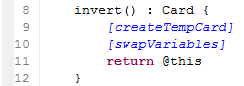
\includegraphics[width=0.4\textwidth]{eclipse_invertControlFlow}
  \caption{Control flow for \texttt{card.invert}}  
  \label{fig:eclipse_invert}
\end{center}
\end{figure}

\item[$\blacktriangleright$] Create two bounded object variables in each pattern, and complete the rules until your patterns resemble
Fig.~\ref{fig:invertPatterns}.

\begin{figure}[htbp]
\begin{center}
  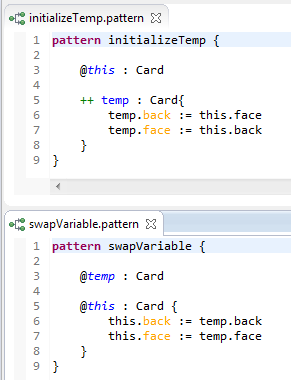
\includegraphics[width=0.5\textwidth]{eclipse_invertPatterns}
  \caption{Swap Patterns}  
  \label{fig:invertPatterns}
\end{center}
\end{figure}

\item[$\blacktriangleright$] Believe it or not, that's it! We reccommend building at this point to confirm nothing has gone wrong with your metamodel. To
see this method in the visual syntax, review Fig.~\ref{fig:sdm_invert}.

\end{itemize}
